\section{Test}
The test setup is an arena with the dimensions 113 x 141 cm as can be seen in figure \ref{fig:testsetup}. The arena is divided into grid cells of 1x1 cm. An obsticle is placed in the middle of the arena to create a unique situation. This enables the robot to locate itself and drive towards a set goal. The map can be seen in figure \ref{fig:map}.
\begin{figure}[H]
\centering
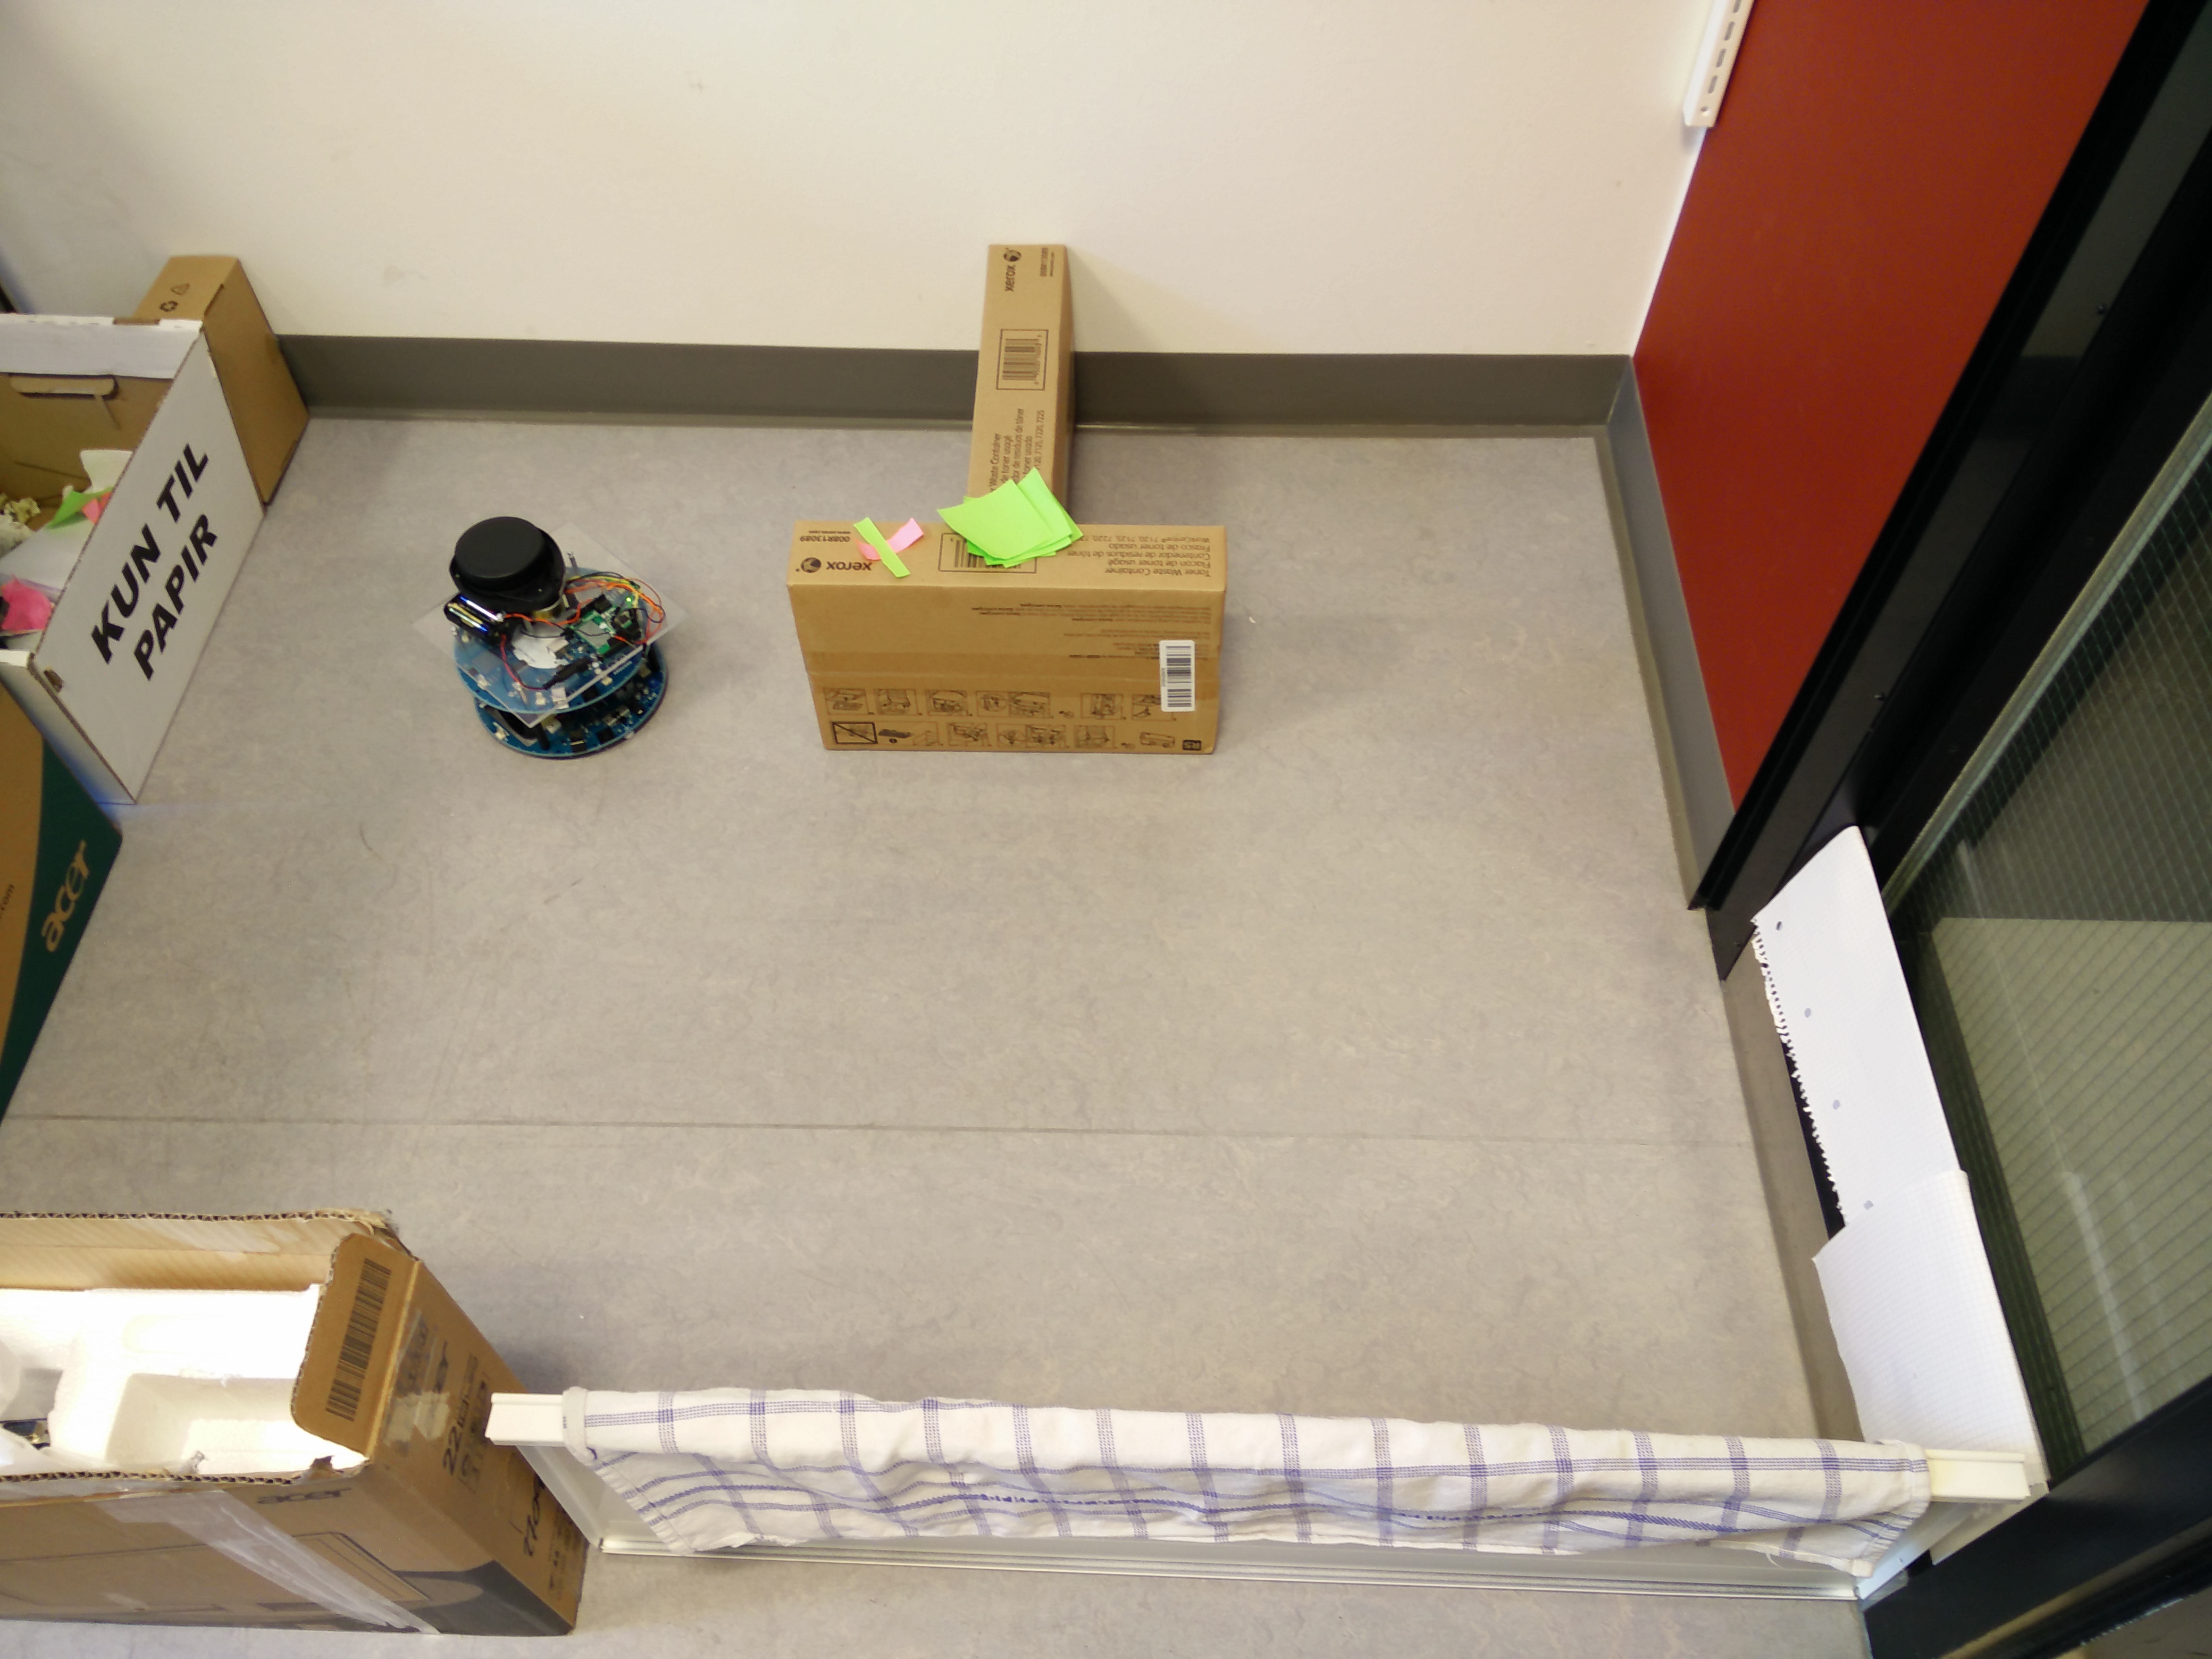
\includegraphics[width=0.8\textwidth]{billeder/testsetup}
\caption{Test Setup}
\label{fig:testsetup}
\end{figure}
\begin{figure}[H]
\centering

\includegraphics[scale=1]{billeder/map}
\caption{Test Map}
\label{fig:map}
\end{figure}